\documentclass[../../main.tex]{subfiles}
\begin{document}
\chapter{Multi-Track and Non-Linear Synthesis}
\label{ch:multi_track}

Human movement is a symphony of coordinated actions, where each part of the body plays a distinct role, yet all work together in harmony to create a seamless expression of intent. The essence of this coordination lies in the ability to perform multiple actions simultaneously or in carefully timed sequences, with each movement contributing to the larger tapestry of physical expression.

Traditional approaches to animating human movement often oversimplify this complexity, reducing it to linear bone rotations. In contrast, multi-track control offers a more nuanced perspective by recognizing the layered, interconnected nature of gestures and postures, reflecting the true complexity of human movement. In the previous chapter, we discussed the creation of an avatar and the generation of signs using AZee \emph{Constraint Scores}. This chapter shifts focus to the animation of the avatar using the AZee \emph{Synced Score} structure. As discussed in section \ref{ch:background_work:sign_language_descriptions:azee} of chapter \ref{ch:background_work}, the AZee Synced Score is a recursive representation of the AZee description, where each block corresponds to a different \emph{linguistic} aspect of the sign. We propose a novel approach to \gls{sl} synthesis using multi-track and non-linear editing techniques. By preserving the dynamics of individual animation blocks, this method enhances reusability, accuracy, and flexibility in the synthesis process.

The content of this chapter is structured as follows. First, Section~\ref{ch:multi_track:related_work} reviews related work in the field of multi-track and non-linear editing, with a focus on their applications in animation and \gls{sl} synthesis. Section~\ref{ch:multi_track:score_to_timeline} introduces the process of converting an AZee Synced Score into a multi-track timeline, outlining the benefits of this representation. Section~\ref{ch:multi_track:azee_nl} explores the implications of non-linear synthesis within the AZee framework, particularly how block evaluation order influences the final animation. In Section~\ref{ch:multi_track:resolve_conflitcs}, we discuss strategies for resolving conflicts between overlapping animation blocks to ensure smooth and accurate motion. Section~\ref{ch:multi_track:second_pass} details the second-pass evaluation process, focusing on cyclic block sets, transpath blocks, and hold blocks to refine the animation. Section~\ref{ch:multi_track:preanim_blocks} addresses the integration of pre-animated blocks into the multi-track timeline, emphasizing both the benefits and challenges of this approach. Finally, Section~\ref{ch:multi_track:implem_results} presents the implementation and results of our multi-track and non-linear synthesis approach, demonstrating improvements in animation quality, flexibility, and procedural generation.

\section{AZee Synced Score to Multi-Track Timeline}
\label{ch:multi_track:score_to_timeline}

todo add constraint block structure

One of the areas which this work aims to address is the direct creation of a multi-track animation timeline from an AZee Synced Score structure. This approach allows for the preservation of the original multi-track information and dynamics present in the AZee description. The algorithm~\ref{alg:azee_timeline} shows how the AZee Synced Score is converted into a multi-track timeline.

\begin{algorithm}
    \caption{AZee Recursion Algorithm (Simplified)}
    \label{alg:azee_timeline}
    \begin{algorithmic}[1]
        \Function{CreateBlocks}{name, score, parent\_name, parent\_score, dynamic\_points}
            \If {parent\_score is not None}
                \State name $\gets$ name + "." + parent\_name
                \State \Call{UpdateSyncRules}{parent\_score, name}
            \EndIf
            
            \State \Call{UpdateBlockTimings}{name, score, parent\_name, parent\_score}
            \If {score.dynamic\_point}
                \State dynamic\_points.append(score.dynamic\_point)
            \EndIf
            
            \If {shortcut\_action $\gets$ \Call{GetShortcutAction}{score} \textbf{and} UseShortcutActions()}
                \State \Return \Call{CreateShortcutBlock}{name, score, parent\_score}
            \ElsIf {score is a SyncedScore}
                \For {child\_name, child\_score in score.block\_contents}
                    \State \Call{CreateBlocks}{child\_name, child\_score, name, score, dynamic\_points}
                \EndFor
            \Else
                \State \Return \Call{CreateRegularBlock}{name, score, parent\_score}
            \EndIf
            
            \If {parent\_score is not None}
                \State \Call{UpdateParentTimings}{parent\_name, name}
            \EndIf
        \EndFunction
    \end{algorithmic}
\end{algorithm}

The figure~\ref{fig:azee_timeline} shows the multi-track timeline generation for \emph{:cupboard}.

\begin{figure}[h]
    \centering
    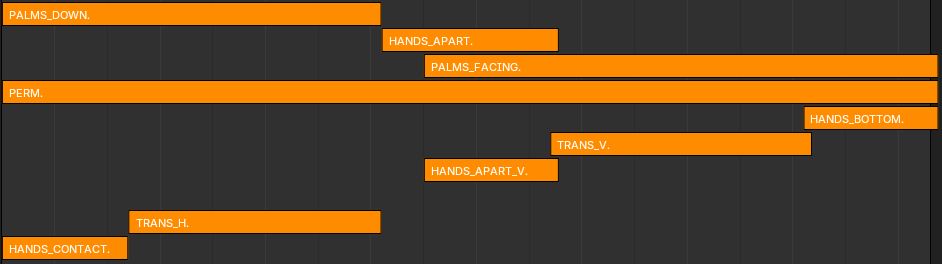
\includegraphics[width=0.8\textwidth]{chapters/multi_track/images/azee_timeline.png}
    \caption{Multi-track timeline generation from an AZee Synced Score.}
    \label{fig:azee_timeline}
\end{figure}


\section{ConstraintDAG}
\label{ch:multi_track:constraint_dag}



The constraints in the blocks can be represented as a Directed Acyclic Graph (DAG) where the nodes are the constraints and the edges represent the dependencies between the constraints. During evaluation, a topological sort enables that no posture constraint is broken. The figure~\ref{fig:constraint_dag_armoire} shows example of a ConstraintDAG for the block HANDS_CONTACT for the sign\emph{armoire} (or cupboard) (sign \emph{armoire} in figure \ref{fig:armoire_sign}). A more complex DAG of constraints can be seen in figure~\ref{fig:constraint_dag_tree} for the sign \emph{tree} (sign tree in figure \ref{fig:tree_sign}).

\begin{figure}[h]
    \centering
    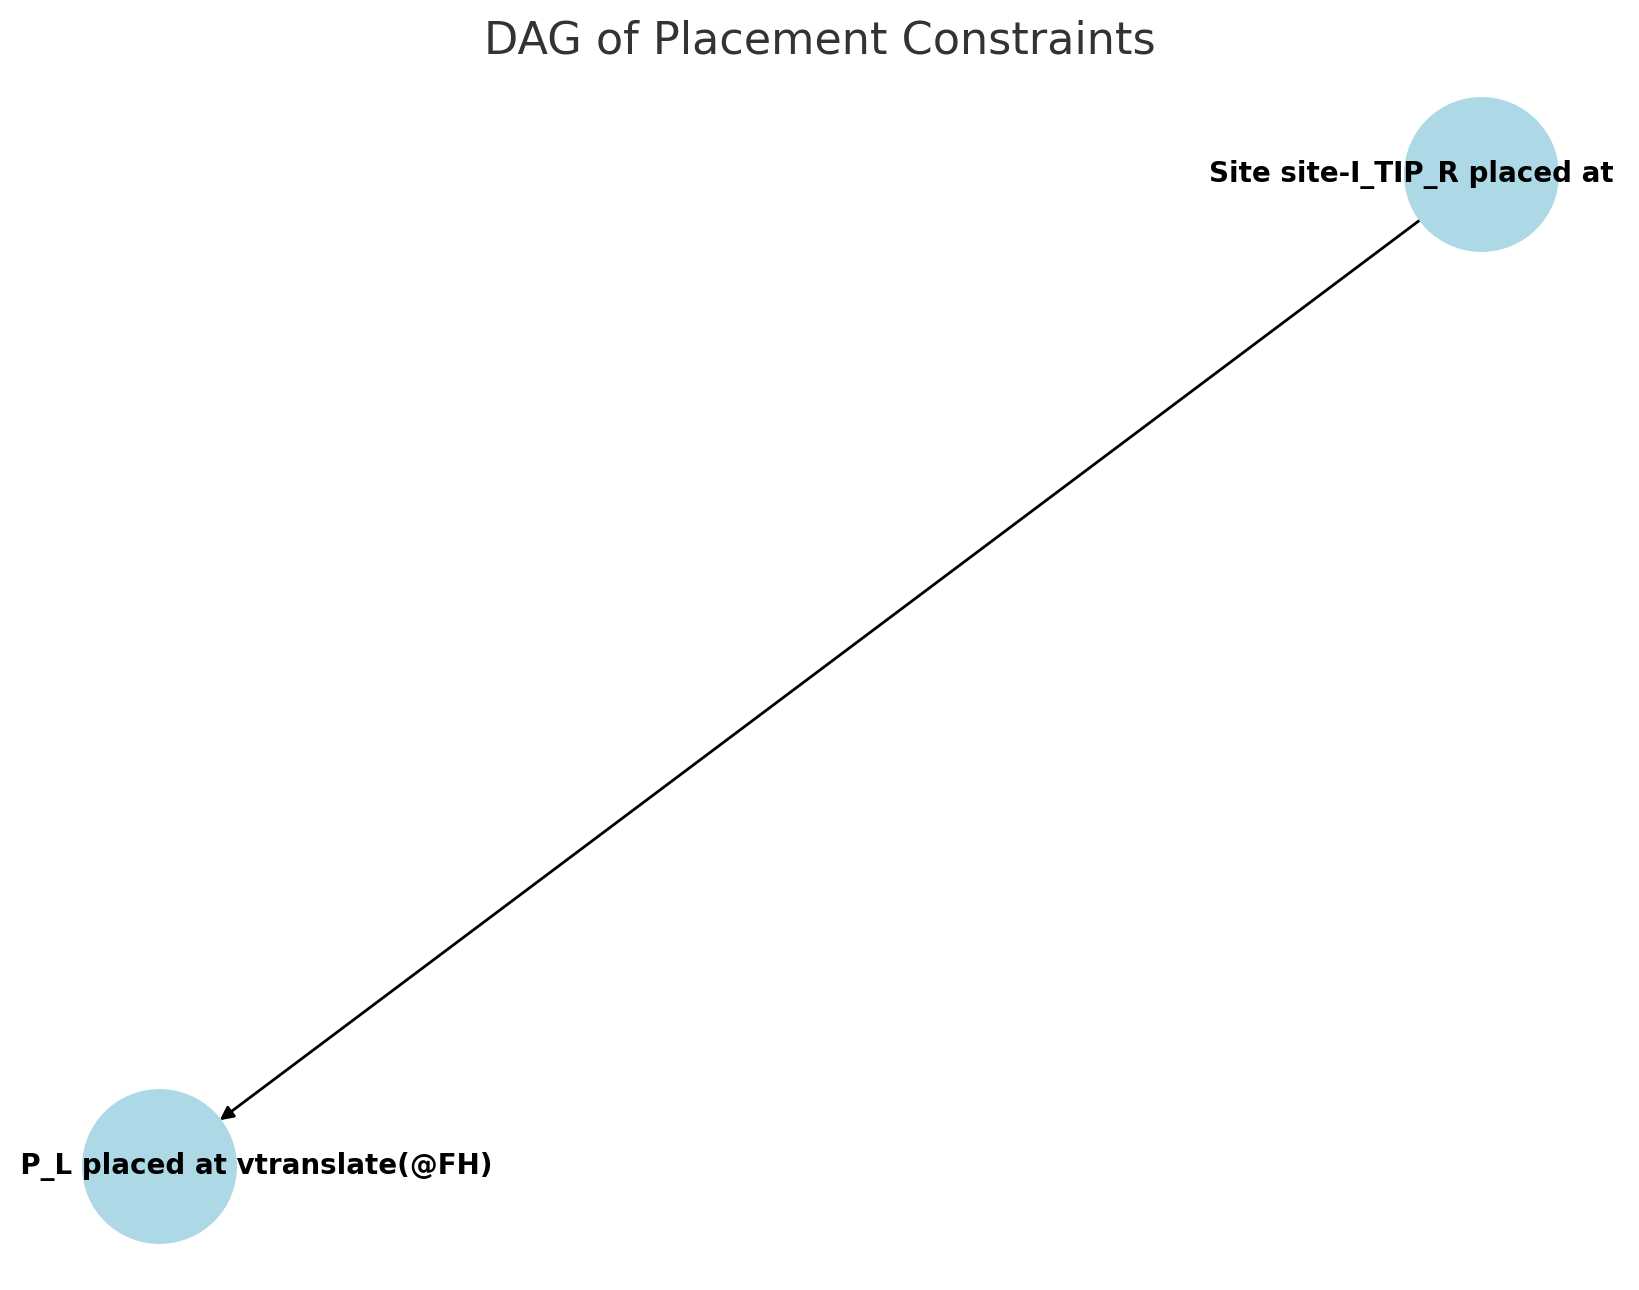
\includegraphics[width=0.8\textwidth]{chapters/multi_track/images/constraint_dag_cupboard.png}
    \caption{ConstraintDAG for a single block discource for the block HANDS\_CONTACT from the sign \emph{cupboard}.}
    \label{fig:constraint_dag_cupboard}
\end{figure}

\begin{figure}
    \centering
    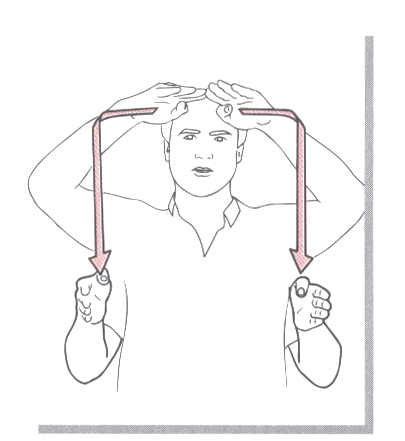
\includegraphics[width=0.8\textwidth]{chapters/multi_track/images/cupboard.jpg}
    \caption{Sign \emph{cupboard}~\cite{moody97}}
    \label{fig:armoire_sign}
\end{figure}

\begin{figure}[h]
    \centering
    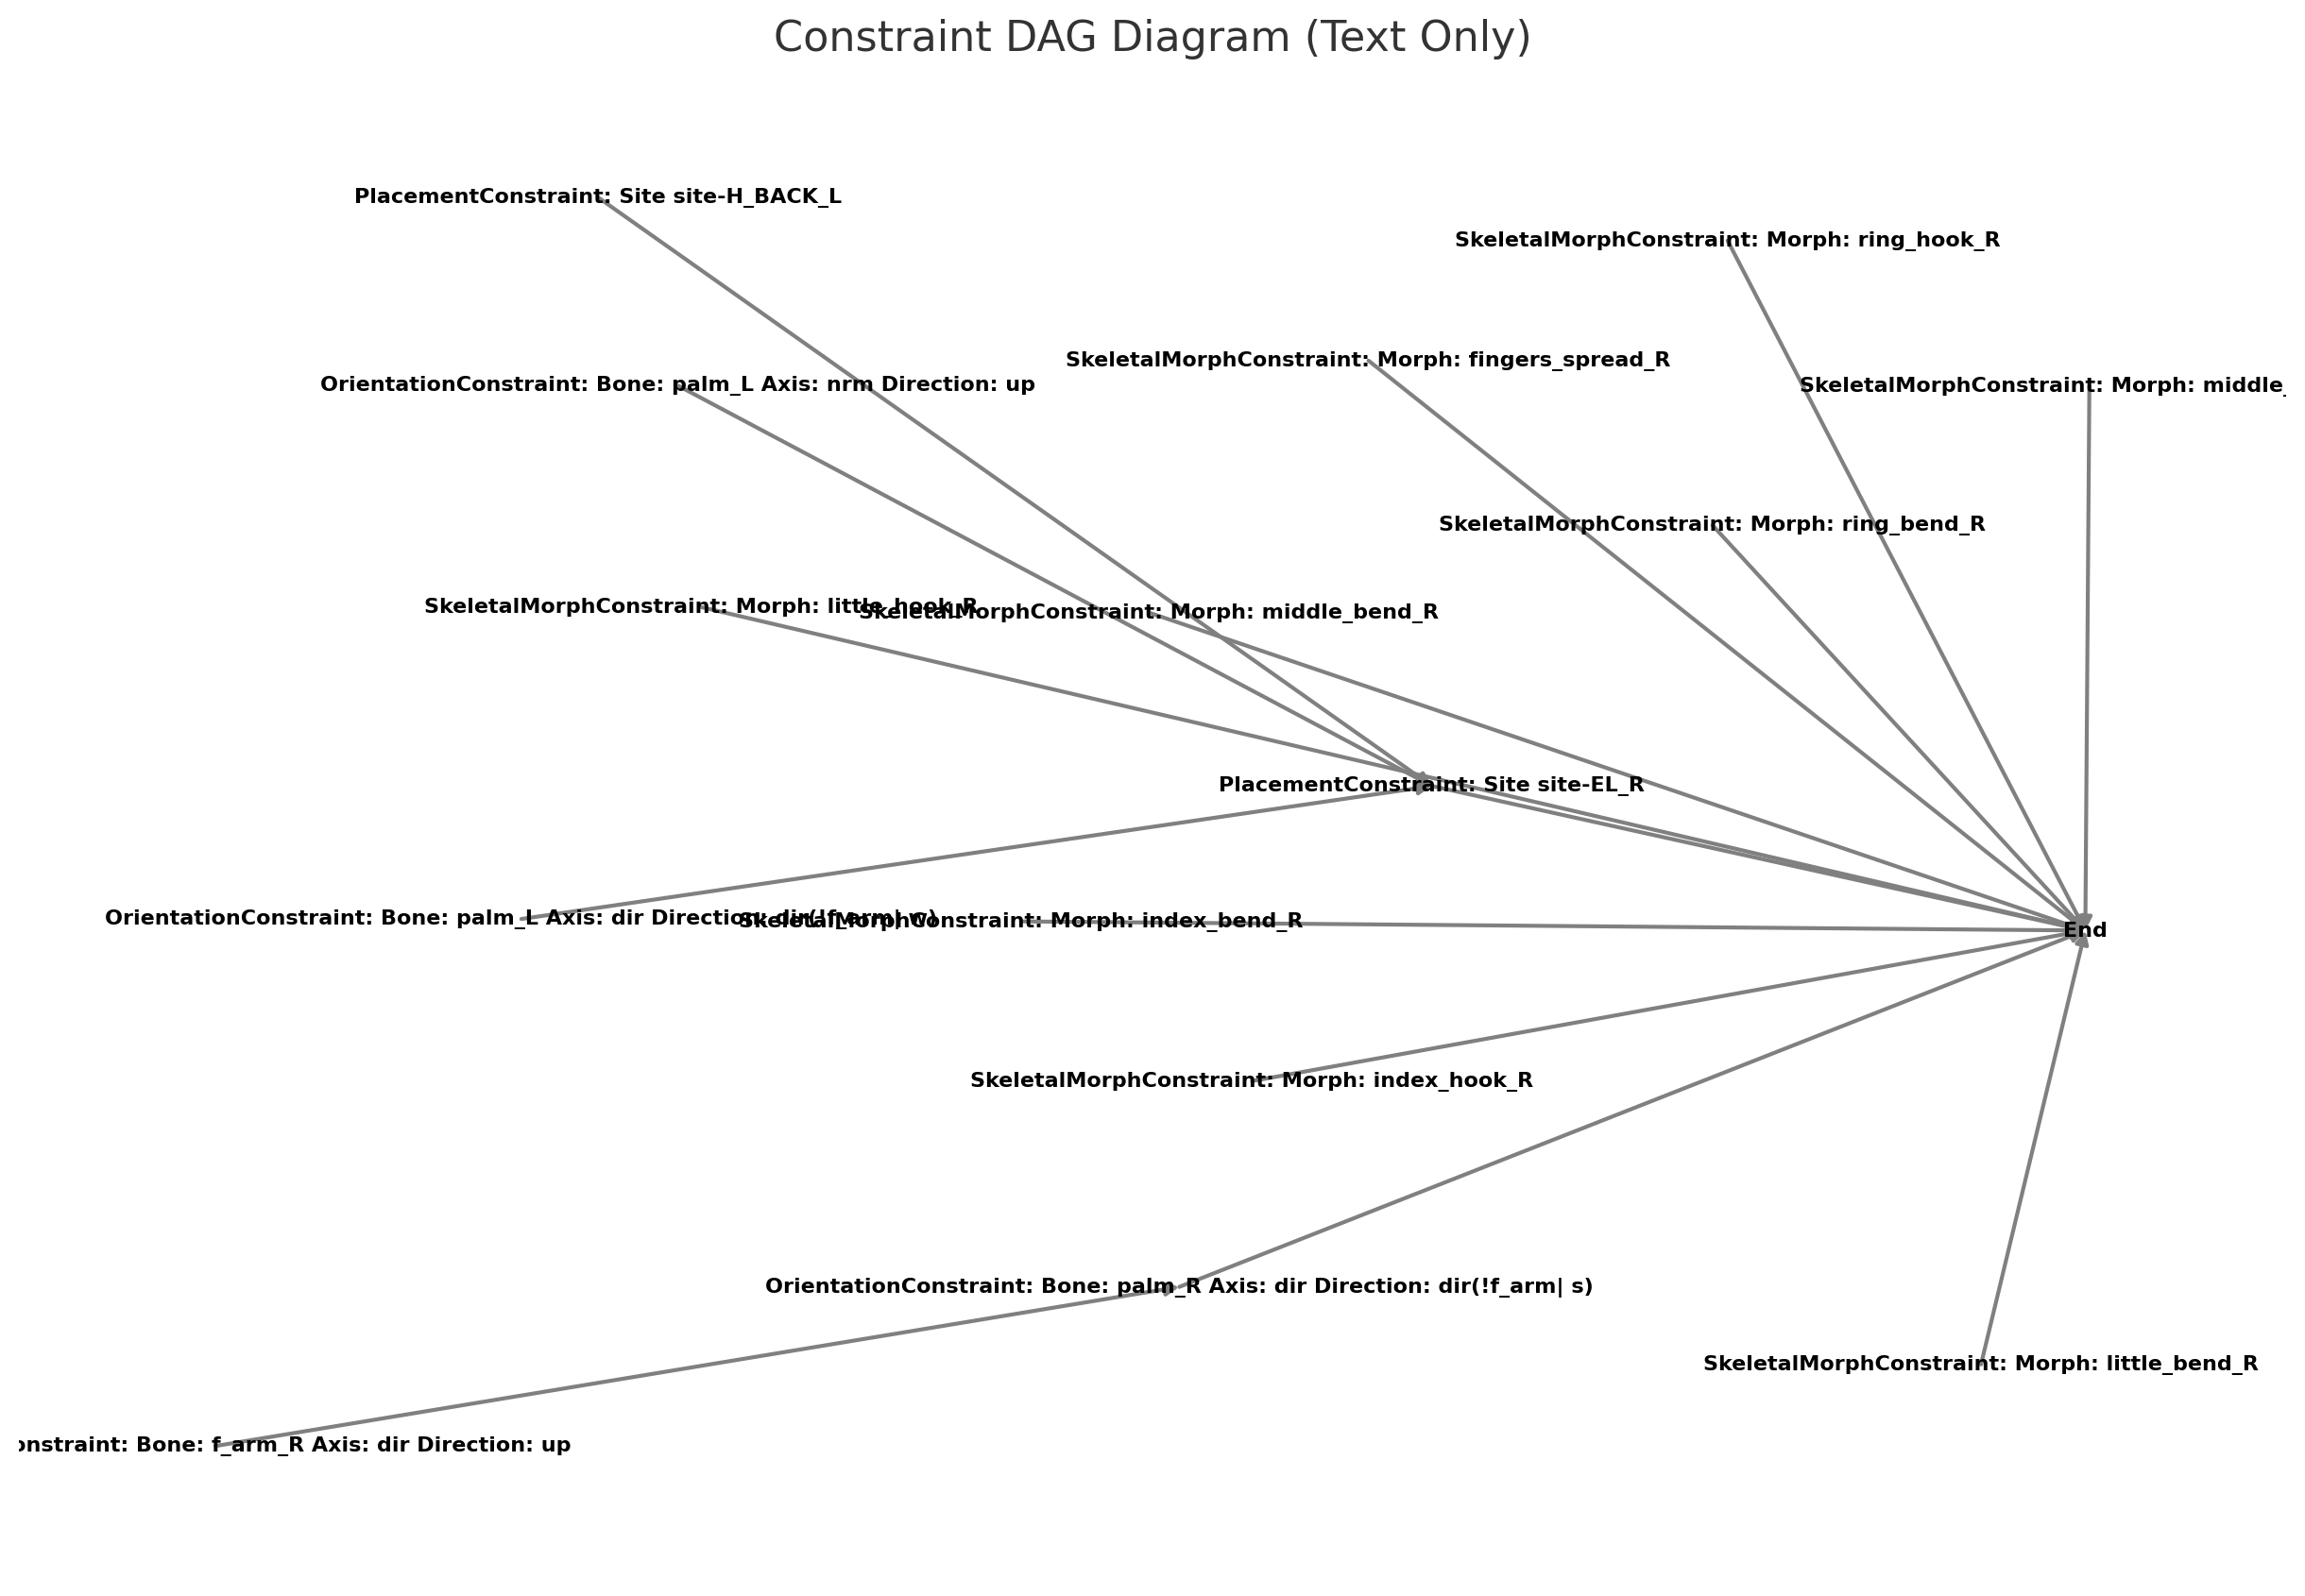
\includegraphics[width=0.8\textwidth]{chapters/multi_track/images/constraint_dag.png}
    \caption{ConstraintDAG for a single block discource for the sign \emph{tree}.}
    \label{fig:constraint_dag_tree}
\end{figure}

\begin{figure}
    \centering
    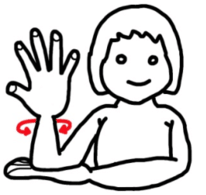
\includegraphics[width=0.8\textwidth]{chapters/multi_track/images/tree.jpg}
    \caption{Sign \emph{tree}}
    \label{fig:tree_sign}
\end{figure}

\section{AZee and Non-Linearity}
\label{ch:multi_track:azee_nl}

The order of synthesis of the blocks in the multi-track timeline is crucial for avoiding conflicts and ensuring the correct execution of constraints. Due to dependencies, an action which happens later in the timeline might be synthesized first. This makes the synthesis non-linear. 

For example, the \emph{transpath} block TRANS\_H in the sign \emph{armoire} is evaluated after the block such as HANDS\_APART for the sign \emph{armoire}. This is because thsi constraint requires resolution of both initial and final position for the hand IK chain. Figure~\ref{fig:example_azee_non_linear} non-linear synthesis for the sign \emph{armoire}.

\begin{figure}[h]
    \centering
    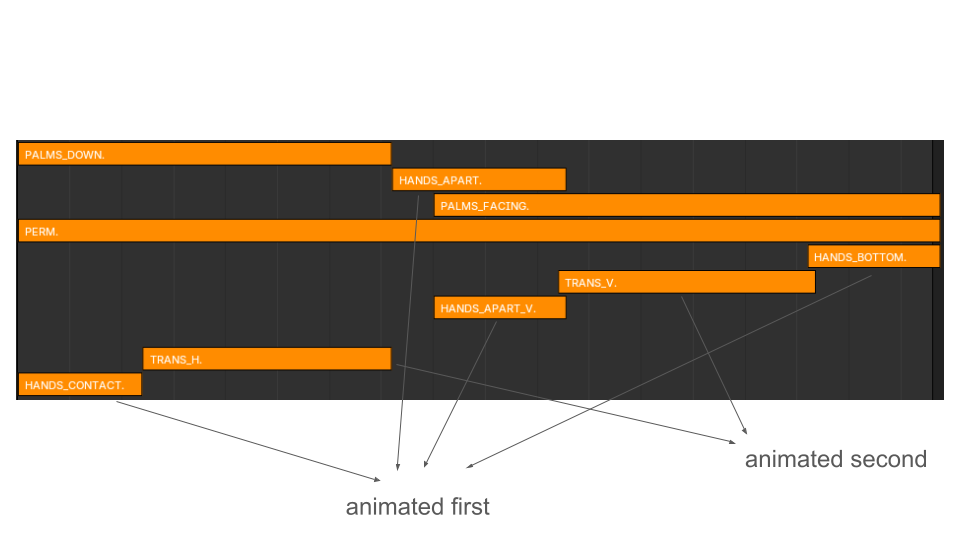
\includegraphics[width=0.8\textwidth]{chapters/multi_track/images/example_azee_non_linear.png}
    \caption{Example of non-linear synthesis in AZee.}
    \label{fig:example_azee_non_linear}
\end{figure}

\section{Resolving Block Conflicts}
\label{ch:multi_track:resolve_conflitcs}

todo fix this

Since the blocks in the multi-track timeline can have constraints that affect the same body parts, conflicts can arise. For example, both blocks PALMS\_DOWN and HANDS\_CONTACT affect both the palm bones. Such conflicts need to be resolved to ensure the correct execution of the constraints. To resolve these conflicts, we use a dependancy graph of constraints for each block \emph{ConstraintDAG} and follow a set of rules to evaluate the blocks.


\subsection{Rule 1: Timely Evaluation}
\label{ch:multi_track:resolve_conflitcs:rule1}

\textbf{Problem:} Overlapping blocks with different start times. \\

\textbf{Example:} Let's consider the timeline in figure~\ref{fig:azee_timeline} for the sign \emph{armoire} (figure~\ref{fig:armoire_sign}). Here, blocks PALMS\_DOWN (palms facing down) and HANDS\_APART (hands being apart) overlap(effect the same bones i.e. the hand chains at the same time).  \\

\textbf{Solution:} Evaluate blocks chronologically to maintain logical sequence i.e. the block that starts first is evaluated first. Thus, the block, PALMS\_DOWN, is evaluated first before the block HANDS\_APART.  \\

\subsection{Rule 2: Constraint Precedence}
\label{ch:multi_track:resolve_conflitcs:rule2}

\textbf{Problem:} Order of topological sorting in case of no constraint dependencies for a block. \\

\textbf{Example:} For same timeline in figure~\ref{fig:azee_timeline}, the block HANDS\_CONTACT containts two constraints, a placement of hands contacting each other at a small distance from the forehead, and the orientation of the wrist along the forearm. Both of these constraints \\

\textbf{Solution:} Follow the constraint precedence order: \emph{placement}, \emph{transpaths}, \emph{lookat}, \emph{trill}, \emph{orientation} and then \emph{morph}The block HANDS\_CONTACT optimizes the posture for placements first, then the orienations of the palm(coming from the block PALMS\_DOWN). . \\

Non-overlapping blocks can be evaluated in parallel since they won't break the posture. Example, blocks PERM and HANDS\_CONTACT is non-overlapping block set in the sign \emph{armoire}.

\section{Second Pass}
\label{ch:multi_track:second_pass}

A second pass is done on the timeline to synthesize cyclic block sets, transpath, and hold blocks.

\subsection{Cyclic Block Set}
\label{ch:multi_track:second_pass:cyclic_blocks}

Cyclic block sets, as the name suggests, are blocks that effect each other cyclically. The figure~\ref{fig:cyclic_blocks} shows a cyclic block set for HANDS\_CONTACT and PALMS\_DOWN. This problem could arise if blocks effect a common heirarchy of the skeleton(any changes in parent will change the child even if the blocks don't effect that part of the skeleton). To deal with such sets, the blocks are evaluated again in a second pass by optimising for a \emph{cumulative flattened loss} i.e. cumulating loss of all constraints of the block set for the frame and optimising them together.

\begin{figure}[h]
    \centering
    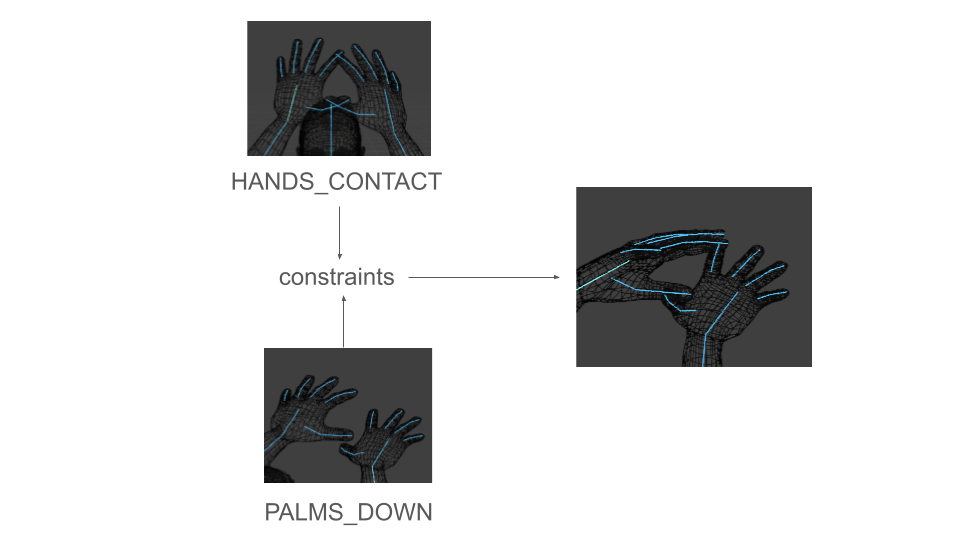
\includegraphics[width=0.8\textwidth]{chapters/multi_track/images/cyclic_blocks.png}
    \caption{Cyclic block set for PALMS\_DOWN and HANDS\_CONTACT}
    \label{fig:cyclic_blocks}
\end{figure}

\subsubsection{Baking Cyclic Blocks}
\label{ch:multi_track:second_pass:cyclic_blocks:baking_cyclic_blocks}

Even though the constraints are optimised together, each individual block in the cyclic block set is baked separately. This is done by collecting the \emph{change in motion curve} of each block and applying them separately to the skeleton after the optimization step (\ref{fig:baking_cyclic_blocks}).

\begin{figure}
    \centering
    \includegraphics[width=0.8\textwidth]{chapters/multi_track/images/baking_cyclic_blocks.png}
    \caption{Baking cyclic block sets}
    \label{fig:baking_cyclic_blocks}
\end{figure}

\subsection{Transpath Blocks}
\label{ch:multi_track:second_pass:transpath_blocks}

Transpath blocks are blocks which contain transpath constraints. A transpath constraint is a constraint that moves a body site along a path. It acts as an interpolation block but with a controlled path for a particular body site for it's preceding block and following blocks. The figure~\ref{fig:transpath_blocks} shows an example of transpath blocks for the sign \emph{cupboard}. Just like cyclic block sets, transpath blocks are evaluated in a second pass.

Transpath blocks are baked by evaluating the transpath constraint for each frame and applying the change in motion curve of the body site wrt to the preceding and the successing block. These motion curves are then baked as a new block.

\begin{figure}[h]
    \centering
    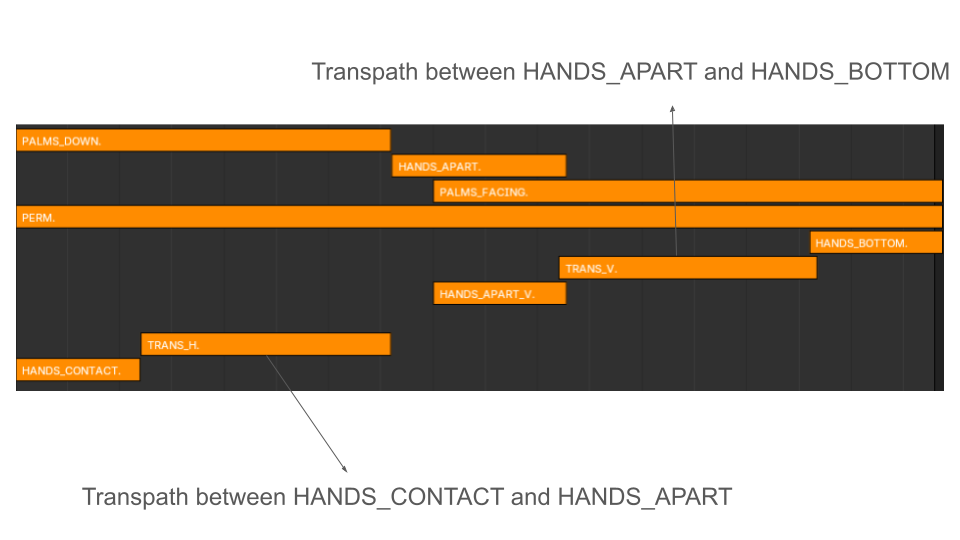
\includegraphics[width=0.8\textwidth]{chapters/multi_track/images/transpath_blocks.png}
    \caption{Transpath blocks in \emph{cupboard}}
    \label{fig:transpath_blocks}
\end{figure}

\subsection{Hold Blocks}
\label{ch:multi_track:second_pass:hold_blocks}

Hold blocks are blocks that hold another block for a certain duration. The figure~\ref{fig:hold_blocks} shows an example of hold blocks for the rule \emph{:info-about(:topic, :info)}. Hold blocks are also evaluated in the second pass since they hold another block(which has to be evaluated in the 1st pass).

Hold blocks are baked by extending the end of the motion curves of the block being held.

\begin{figure}
    \centering
    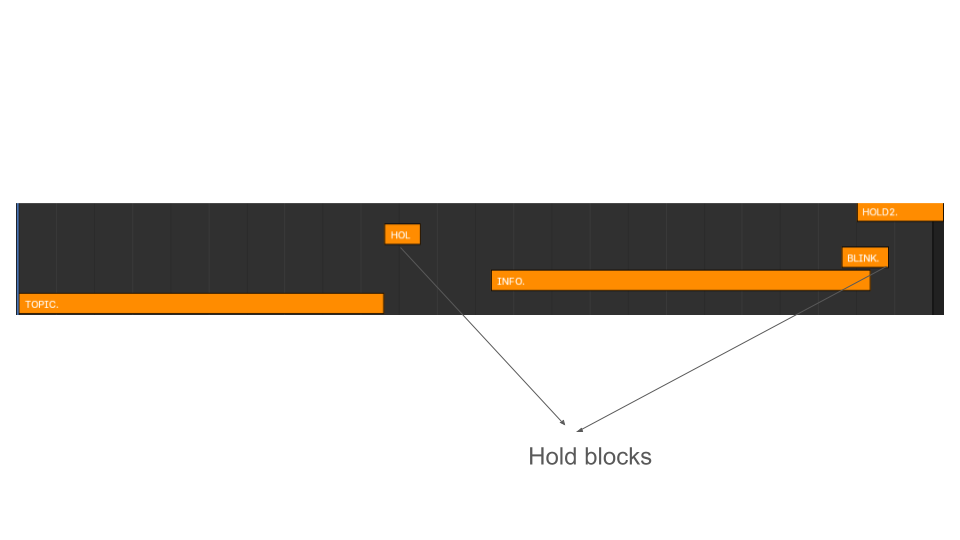
\includegraphics[width=0.8\textwidth]{chapters/multi_track/images/hold_blocks.png}
    \caption{Hold blocks for the rule \emph{:info-about(:topic, :info)}.}
    \label{fig:hold_blocks}
\end{figure}

\section{Pre-animated blocks}
\label{ch:multi_track:preanim_blocks}

The timeline can also contain pre-animated blocks. These blocks are blocks that contain pre-animated motion data. The pre-animated blocks are evaluated and baked first since they are independant of other blocks (figure~\ref{fig:preanim_blocks}).

\begin{figure}[h]
    \centering
    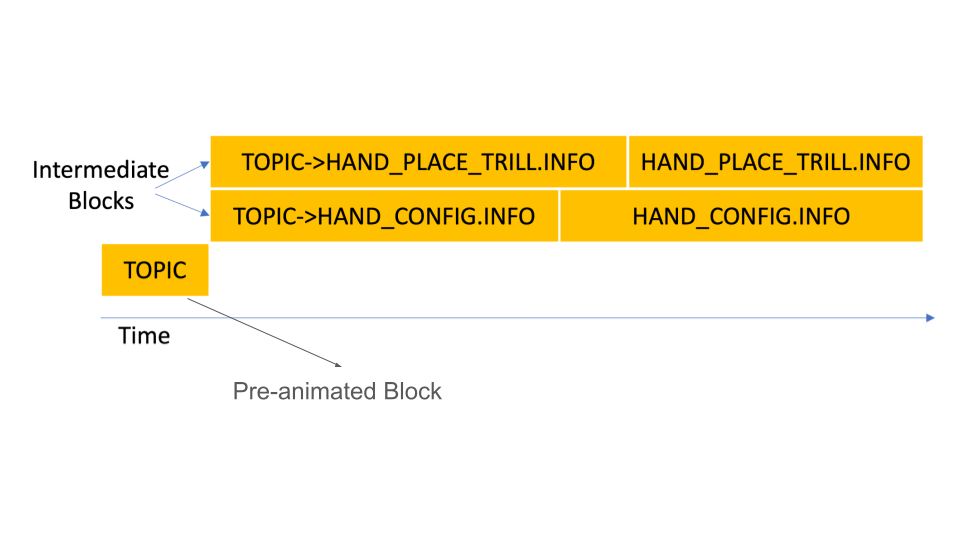
\includegraphics[width=0.8\textwidth]{chapters/multi_track/images/preanim_blocks.png}
    \caption{Pre-animated blocks in the multi-track timeline.}
    \label{fig:preanim_blocks}
\end{figure}

\section{Implementation and Results}
\label{ch:multi_track:implem_results}

The multi-track timeline is implementated in blender's non-linear editor. Each AZee Score, when animated, generates a blender action which is put on the non-linear editor as a strip with duration specified by the AZee \emph{sync rules}. The following table~\ref{tab:azee_to_blender} shows a non-exhaustive list of animated signs in blender with their corresponding generated timeline.

\begin{table}[h]
    \centering
    \begin{tabular}{|c|c|}
        \hline
        \textbf{Sign} & \textbf{Timeline} \\
        \hline
        \emph{tree} & figure todo \\
        \emph{cupboard} & figure todo \\
        \emph{...} & ... \\
        \hline
    \end{tabular}
    \caption{Animated signs in blender with their corresponding generated timeline.}
    \label{tab:azee_to_blender}
\end{table}

\section{Discussion}
\label{ch:multi_track:discussion}

The multi-track timeline approach to \gls{sl} synthesis offers several advantages over the existing existing method. Preserving the multi-track information and dynamics present in the AZee description provides us the stepping stones to integrate pre-animated motion data which was not possible with the previous low-level AZee synthesizor. The non-linear synthesis allows for the correct execution order of blocks and avoids conflicts. On top of that, hybrid constucts such as \emph{dynamic points} (a point changing it's location over time) can be easily integrated into the timeline (figure~\ref{fig:dynpoint_example}).

\begin{figure}[h]
    \centering
    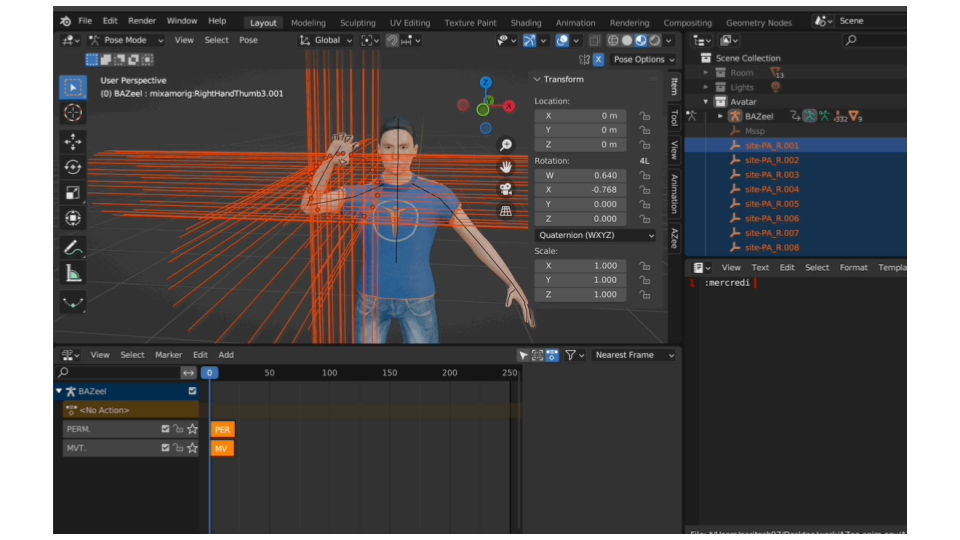
\includegraphics[width=0.8\textwidth]{chapters/multi_track/images/dynpoint_example.png}
    \caption{Example of a dynamic point in the multi-track timeline.}
    \label{fig:dynpoint_example}
\end{figure}

\end{document}
